% ------------------------------------------------------------
% File: figures/fig-interleaved-quadrants.tex
% Interleaved recess depths across two samples
% ------------------------------------------------------------

\begin{figure}[htbp]
  \centering
  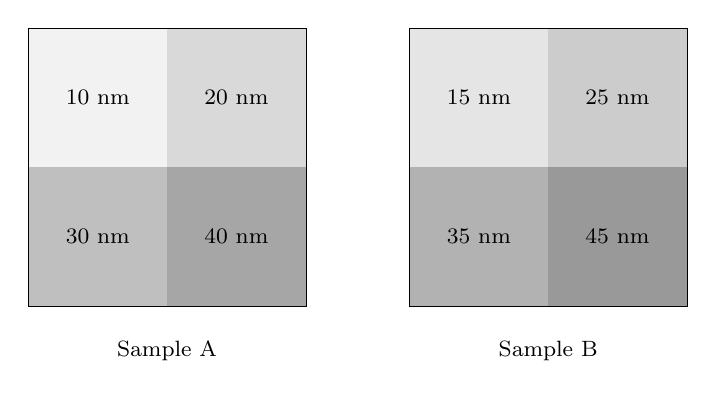
\begin{tikzpicture}[x=1.1cm, y=1.1cm, font=\footnotesize]
    % Parameters
    \def\cell{1.6}
    \def\gap{1.2}
    \def\labely{-0.3}

    % Sample A (left)
    \begin{scope}
      \draw[line width=0.6pt] (0,0) rectangle (2*\cell,2*\cell);
      \draw[line width=0.6pt] (\cell,0) -- (\cell,2*\cell);
      \draw[line width=0.6pt] (0,\cell) -- (2*\cell,\cell);
      \fill[gray!10] (0,\cell) rectangle (\cell,2*\cell);
      \fill[gray!30] (\cell,\cell) rectangle (2*\cell,2*\cell);
      \fill[gray!50] (0,0) rectangle (\cell,\cell);
      \fill[gray!70] (\cell,0) rectangle (2*\cell,\cell);
      \node at (0.5*\cell,1.5*\cell) {10 nm};
      \node at (1.5*\cell,1.5*\cell) {20 nm};
      \node at (0.5*\cell,0.5*\cell) {30 nm};
      \node at (1.5*\cell,0.5*\cell) {40 nm};
      \node[anchor=north] at (\cell,\labely) {Sample A};
    \end{scope}

    % Sample B (right)
    \begin{scope}[shift={({2*\cell+\gap},0)}]
      \draw[line width=0.6pt] (0,0) rectangle (2*\cell,2*\cell);
      \draw[line width=0.6pt] (\cell,0) -- (\cell,2*\cell);
      \draw[line width=0.6pt] (0,\cell) -- (2*\cell,\cell);
      \fill[gray!20] (0,\cell) rectangle (\cell,2*\cell);
      \fill[gray!40] (\cell,\cell) rectangle (2*\cell,2*\cell);
      \fill[gray!60] (0,0) rectangle (\cell,\cell);
      \fill[gray!80] (\cell,0) rectangle (2*\cell,\cell);
      \node at (0.5*\cell,1.5*\cell) {15 nm};
      \node at (1.5*\cell,1.5*\cell) {25 nm};
      \node at (0.5*\cell,0.5*\cell) {35 nm};
      \node at (1.5*\cell,0.5*\cell) {45 nm};
      \node[anchor=north] at (\cell,\labely) {Sample B};
    \end{scope}
  \end{tikzpicture}

  \vspace{2mm}
  \caption{Interleaved allocation of recess depths across the four quadrants of two samples.}
  \label{fig:interleaved_quadrants}
\end{figure}
